\documentclass[journal,12pt,twocolumn]{IEEEtran}

\usepackage{setspace}
\usepackage{gensymb}
\singlespacing
\usepackage[cmex10]{amsmath}
\usepackage{amssymb}
\usepackage{xurl}

\usepackage{amsthm}
\usepackage{comment}
\usepackage{mathrsfs}
\usepackage{txfonts}
\usepackage{stfloats}
\usepackage{bm}
\usepackage{cite}
\usepackage{cases}
\usepackage{subfig}

\usepackage{longtable}
\usepackage{multirow}

\usepackage{enumitem}
\usepackage{mathtools}
\usepackage{steinmetz}
\usepackage{tikz}
\usepackage{circuitikz}
\usepackage{verbatim}
\usepackage{tfrupee}
\usepackage[breaklinks=true]{hyperref}
\usepackage{graphicx}
\usepackage{tkz-euclide}

\usetikzlibrary{calc,math}
\usepackage{listings}
    \usepackage{color}                                            %%
    \usepackage{array}                                            %%
    \usepackage{longtable}                                        %%
    \usepackage{calc}                                             %%
    \usepackage{multirow}                                         %%
    \usepackage{hhline}                                           %%
    \usepackage{ifthen}                                           %%
    \usepackage{lscape}     
\usepackage{multicol}
\usepackage{chngcntr}

\DeclareMathOperator*{\Res}{Res}

\renewcommand\thesection{\arabic{section}}
\renewcommand\thesubsection{\thesection.\arabic{subsection}}
\renewcommand\thesubsubsection{\thesubsection.\arabic{subsubsection}}

\renewcommand\thesectiondis{\arabic{section}}
\renewcommand\thesubsectiondis{\thesectiondis.\arabic{subsection}}
\renewcommand\thesubsubsectiondis{\thesubsectiondis.\arabic{subsubsection}}


\hyphenation{op-tical net-works semi-conduc-tor}
\def\inputGnumericTable{}                                 %%

\lstset{
%language=C,
frame=single, 
breaklines=true,
columns=fullflexible
}
\begin{document}


\newtheorem{theorem}{Theorem}[section]
\newtheorem{problem}{Problem}
\newtheorem{proposition}{Proposition}[section]
\newtheorem{lemma}{Lemma}[section]
\newtheorem{corollary}[theorem]{Corollary}
\newtheorem{example}{Example}[section]
\newtheorem{definition}[problem]{Definition}

\newcommand{\BEQA}{\begin{eqnarray}}
\newcommand{\EEQA}{\end{eqnarray}}
\newcommand{\define}{\stackrel{\triangle}{=}}
\bibliographystyle{IEEEtran}
\raggedbottom
\setlength{\parindent}{0pt}
\providecommand{\mbf}{\mathbf}
\providecommand{\pr}[1]{\ensuremath{\Pr\left(#1\right)}}
\providecommand{\qfunc}[1]{\ensuremath{Q\left(#1\right)}}
\providecommand{\sbrak}[1]{\ensuremath{{}\left[#1\right]}}
\providecommand{\lsbrak}[1]{\ensuremath{{}\left[#1\right.}}
\providecommand{\rsbrak}[1]{\ensuremath{{}\left.#1\right]}}
\providecommand{\brak}[1]{\ensuremath{\left(#1\right)}}
\providecommand{\lbrak}[1]{\ensuremath{\left(#1\right.}}
\providecommand{\rbrak}[1]{\ensuremath{\left.#1\right)}}
\providecommand{\cbrak}[1]{\ensuremath{\left\{#1\right\}}}
\providecommand{\lcbrak}[1]{\ensuremath{\left\{#1\right.}}
\providecommand{\rcbrak}[1]{\ensuremath{\left.#1\right\}}}
\theoremstyle{remark}
\newtheorem{rem}{Remark}
\newcommand{\sgn}{\mathop{\mathrm{sgn}}}
\providecommand{\abs}[1]{\vert#1\vert}
\providecommand{\res}[1]{\Res\displaylimits_{#1}} 
\providecommand{\norm}[1]{\lVert#1\rVert}
%\providecommand{\norm}[1]{\lVert#1\rVert}
\providecommand{\mtx}[1]{\mathbf{#1}}
\providecommand{\mean}[1]{E[ #1 ]}
\providecommand{\fourier}{\overset{\mathcal{F}}{ \rightleftharpoons}}
%\providecommand{\hilbert}{\overset{\mathcal{H}}{ \rightleftharpoons}}
\providecommand{\system}{\overset{\mathcal{H}}{ \longleftrightarrow}}
	%\newcommand{\solution}[2]{\textbf{Solution:}{#1}}
\newcommand{\solution}{\noindent \textbf{Solution: }}
\newcommand{\cosec}{\,\text{cosec}\,}
\providecommand{\dec}[2]{\ensuremath{\overset{#1}{\underset{#2}{\gtrless}}}}
\newcommand{\myvec}[1]{\ensuremath{\begin{pmatrix}#1\end{pmatrix}}}
\newcommand{\mydet}[1]{\ensuremath{\begin{vmatrix}#1\end{vmatrix}}}
\numberwithin{equation}{subsection}
\makeatletter
\@addtoreset{figure}{problem}
\makeatother
\let\StandardTheFigure\thefigure
\let\vec\mathbf
\renewcommand{\thefigure}{\theproblem}
\def\putbox#1#2#3{\makebox[0in][l]{\makebox[#1][l]{}\raisebox{\baselineskip}[0in][0in]{\raisebox{#2}[0in][0in]{#3}}}}
     \def\rightbox#1{\makebox[0in][r]{#1}}
     \def\centbox#1{\makebox[0in]{#1}}
     \def\topbox#1{\raisebox{-\baselineskip}[0in][0in]{#1}}
     \def\midbox#1{\raisebox{-0.5\baselineskip}[0in][0in]{#1}}
\vspace{3cm}
\title{AI1103 : Assignment 2}
\author{Yashas Tadikamalla - AI20BTECH11027}
\maketitle
\newpage
\bigskip
\renewcommand{\thefigure}{\theenumi}
\renewcommand{\thetable}{\theenumi}
Download all python codes from 
\begin{lstlisting}
https://github.com/YashasTadikamalla/AI1103/tree/main/Assignment2/codes
\end{lstlisting}
%
and latex codes from 
%
\begin{lstlisting}
https://github.com/YashasTadikamalla/AI1103/blob/main/Assignment2/Assignment2.tex
\end{lstlisting}
\section*{Problem(5.25)}
A bag contains 2 white and 1 red balls. One ball is drawn at random and then put back in the box after noting its colour. The process is repeated again. If X denotes the number of red balls recorded in the two draws, describe X.

\section*{Solution(5.25)}
Given, a bag containing 2 white and 1 red balls. Let the random variable $X_{i}\in\{0,1\},i=1,2,$ represent the outcome of the colour of the ball drawn in the first, second attempts. $X_{i}=0,X_{i}=1$ denote a white ball, red ball being drawn respectively, in the $i^{th}$ attempt.
\newline
\newline
As the ball drawn in the first attempt is replaced in the bag, for both the attempts, the number of balls of a specified colour, and their probability  mass function's (pmf's) remain the same. i.e, 
\begin{align}
    \tag{5.25.1}
    n(X_{i}=0)=2\\
    \tag{5.25.2}
    n(X_{i}=1)=1\\
    \tag{5.25.3}
    \therefore n(X_{i}=0)+n(X_{i}=1)=3 
\end{align}
and
\begin{align}
    \tag{5.25.4}
    \Pr(X_{i}=j) = 
	\begin{cases}
	\dfrac{2}{3}, &j=0 \\~\\[-1em]
	\dfrac{1}{3}, &j=1 \\~\\[-1em]
	0, & otherwise
	\end{cases}
\end{align}
\newpage
Define 
\begin{align}
    \tag{5.25.5}
    X=X_{1}+X_{2}
\end{align}
so that $X\in\{0,1,2\}$ represents a random variable denoting the number of red balls drawn in both the attempts. Then, $X$ has a binomial distribution with 
\begin{align}
    \tag{5.25.6}
    Pr(X=k)={n\choose k}p^{k}q^{n-k}
\end{align}
where,
\begin{align}
    \tag{5.25.7}
    n=2
\end{align}
\newline $p =$ probability of success = probability of drawing a red ball = $Pr(X_{i}=1)$
\begin{align}
    \tag{5.25.8}
    p=\frac{1}{3}
\end{align}
\newline $q =$ probability of failure = $1-p$
\begin{align}
    \tag{5.25.9}
    q=1-p=1-\frac{1}{3}=\frac{2}{3}
\end{align}
Hence, on substituting and simplifying, we get
\begin{align}
    \tag{5.25.10}
    Pr(X=0)=\frac{4}{9},Pr(X=1)=\frac{4}{9},Pr(X=2)=\frac{1}{9}
\end{align}
Therefore, the pmf for $X$ (theoretical) is
\begin{align}
    \tag{5.25.11}
    \Pr(X=i) = 
	\begin{cases}
	\dfrac{4}{9}, & i=0 \\~\\[-1em]
	\dfrac{4}{9}, & i=1 \\~\\[-1em]
	\dfrac{1}{9}, & i=2 \\~\\[-1em]
	0, & otherwise
	\end{cases}
\end{align}
\newline
\newline
\begin{tabular}{|c|c|c|c|}
    \hline
    Condition & $X = 0$& $X =1 $& $X=2$ \\
    \hline
    Probability & ${2\choose 0}p^{0}q^{2}$ & ${2\choose 1}p^{1}q^{1}$ & ${2\choose 2}p^{2}q^{0}$\\
    \hline
\end{tabular}
\newpage
So, if we conduct this experiment 9000 times, theoretically, we get 
\newline
\newline
\newline
\begin{tabular}{|c|c|c|c|}
    \hline
    Condition & $X = 0$& $X =1 $& $X=2$ \\
    \hline
    Frequency & 4000 & 4000 & 1000\\
    \hline
\end{tabular}
\newline
\newline
\newline
Here are the plots describing $X$, after the experiment is conducted 9000 times.
\newline
\newline
Theoretical vs Simulation
\newline
\newline
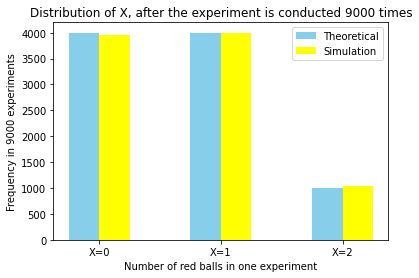
\includegraphics[scale=0.6]{Assignment2(1).png}
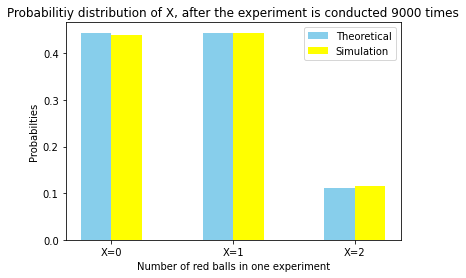
\includegraphics[scale=0.6]{Assignment2(2).png}
\end{document}